\documentclass[a4paper,12pt]{article}
\usepackage{blindtext}
\usepackage[utf8]{inputenc}
\usepackage{graphicx}

\begin{document}
\begin{titlepage}
\center

\textsc{\LARGE Project: Network Visualization}\\[1.5cm]
\textsc{\Large Client: Amazon Web Services}\\[0.5cm]
\textsc{\large Team: Quadcore Productions}\\[0.5cm]

\begin{minipage}{0.4\textwidth}
\begin{flushleft} \large
\emph{Author(s):}\\
Mpho \textsc{Baloyi}\\
Hlengekile \textsc{Jita}\\
Mayimela \textsc{Moses}\\
Mbhele \textsc{Themba}\\
\end{flushleft}
\end{minipage}
~
\begin{minipage}{0.4\textwidth}
\begin{flushright} \large
\emph{Student number(s):} \\
14133670\\ % Student number
14077893\\
14019702\\
14007950\\
\end{flushright}
\end{minipage}\\

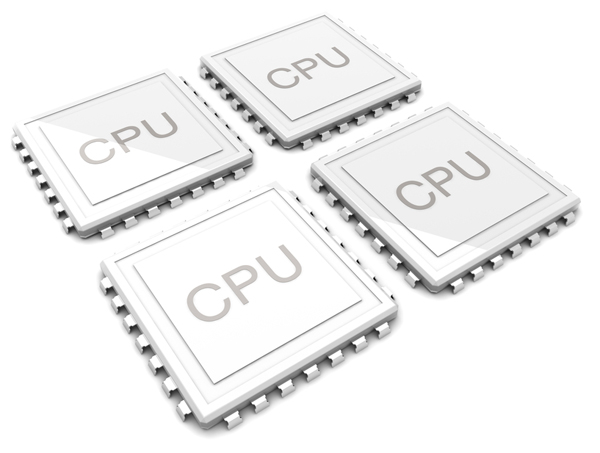
\includegraphics[width=\textwidth]{2012-quad-core-phones}

{\large University of Pretoria, Department of Computer Science}\\

{\large 02 May 2016}\\[3cm]

\vfil

\end{titlepage}

\newpage

\section{The Team}
\subsection{Mpho Baloyi}
\subsubsection{Interests}
\begin{itemize}
\item Keeping abreast with new technologies
\item Learning and using new technologies to solve problems
\item Reading up and doing research on new and old concepts in computer science
\item Solving riddles and puzzles
\item Helping people through ICT
\end{itemize}
\subsubsection{Technical Skills}
\begin{itemize}
\item Solid programming skills in java,c++ and python
\item Fair amount of knowledge in assembly programming
\item Web development with HTML,JAVASCRIPT,JQUERY,CSS,PHP,AJAX,ANGULARJS
\item Interaction Design
\item Database design with MySQL
\item Understanding of process development
\item Unit testing,mocking and dependency Injection
\end{itemize}
\subsubsection{Non-Technical Strengths}
\begin{itemize}
\item Excellent Communication skills
\item Patient
\item Creative approach to problem solving
\item Pay attention to detail
\item Excellent planning skills
\item Ability to grasp concepts quickly
\item Willingness to learn new things
\item Ability to interpret and follow technical plans
\item Ability to collaborate and work efficiently with other people
\item Ability to work under pressure
\end{itemize}
\subsubsection{Relevant Past Experiences}
\subsubsection{Reasons for wanting to do the project}
\begin{flushleft}
My interest and deep passion for Internet of Things,helping people and more importantly providing people with means to take
care of the environment through careful power consumption are the main reasons why I want to do this project. I also want to do
this project because it is an opportunity to learn and see how software and hardware work together which has always been one of my many interests.The project presents an opportunity to learn new things,acquire new skills and refine my skills and I believe this is the head-start I need for my career in Computer Science.
\end{flushleft}
\subsection{Hlengekile Jita}
%\includegraphics[width=\textwidth]{}
\subsubsection{Interests}
\subsubsection{Technical Skills}
\subsubsection{Non-Technical Strengths}
\subsubsection{Relevant Past Experiences}
\subsubsection{Reasons for wanting to do the project}
\subsection{Moses Mayimela}
%\includegraphics[width=\textwidth]{}
\subsubsection{Interests}
\subsubsection{Technical Skills}
\subsubsection{Non-Technical Strengths}
\subsubsection{Relevant Past Experiences}
\subsubsection{Reasons for wanting to do the project}
\subsection{Themba Mbhele}
%\includegraphics[width=\textwidth]{}
\subsubsection{Interests}
\subsubsection{Technical Skills}
\subsubsection{Non-Technical Strengths}
\subsubsection{Relevant Past Experiences}
\subsubsection{Reasons for wanting to do the project}

\section{Project Execution}
\subsection{Project Development Methodology}
\label{Project Design Methodology}
\subsubsection{Data Collection}
The first step is to retrieve the network data. The information may be retrieved from a file or web source.
\subsubsection{Data Classification}
The data will now be validated for correctness. If the data is valid, the different members of the network (parent node, sub-parent node and leaf nodes)
will be identified and classified accordingly. To arrange the data, data structures such as trees will be used.\\
The members of the network that have been identified are:
\begin{itemize}
	\item \textbf{Parent node:} This is the member from which all the other members will be referenced (This is the Main parent or root node).
	\item \textbf{Sub-Parent node:} This is a member that is referenced from another member and has other members that are referenced through it (It is a child with children).
	\item \textbf{Leaf node:} This member is at the lowest level of the tree data structure, it is referenced through a parent and has no members that are referenced through it ( It has no children).
\end{itemize}
\newpage
\subsubsection{Data visualization}
After all the data has been retrieved successfully and the members classified to the respective types, the data will then be loaded to the screen for visual representation (visualize). At this stage, the data can be viewed while allowing interactions for the user. The interactions will include zooming in and out of the visualizer,panning around the graph, click events for more information on a specific member of the network.\\ \\
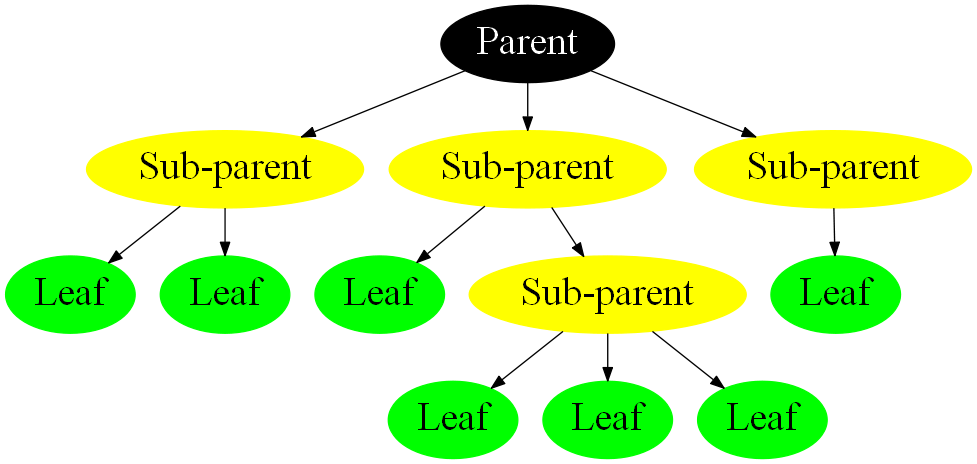
\includegraphics[width=\textwidth]{images/graph1.png}
\begin{center}
Data organization as data structure and basic representation
\end{center}
The image above is a basic representation of how data structures will be used to organize the data and also a starting point as to how the data will be visualized.
\subsection{Communication With Client}
To keep the clients informed we are going to use the following means of communication
\subsubsection{email}
\begin{itemize}
\item To inform the client of our progress
\item To address any issues or concerns that they client may have
\item To acquire information from the client
\item To require any resources that the client has to offer for their project,..
\end{itemize}
\subsubsection{Phone calls}
This will only be used to address very urgent matters if they arise during the course of the project development
however this will only be done with permission from the client and during business hours.
\subsubsection{Regular Meetings}
These will take place depending on the clients availiability and willness.
We may discuss the progress of the project,to address any concerns,etc.
\subsubsection{GIT}
Access to our git repository will be provided to the client,so the client can be able to monitor
our progress and have access to the project material.
We are also open to any means of communicatiuon that the client may prefer or suggest.
\subsection{Technical Challenges}
\begin{itemize}
\item Learning the EC2 API 

As this is a very specific technology and one that we have not encountered before but we have a strong believe that 
through more research,more information from the client and our previous experiences with using an API we can overcome this challenge.

\item Retrieving Data from Amazon

This challenge is only due to the lack of information at this stage we plan to overcome this challenge by using either xml or JSON.
\end{itemize}
\subsection{Technologies}
\end{document}
